\documentclass[conference]{IEEEtran}
\usepackage[T1]{fontenc}
\usepackage[utf8]{inputenc}
\usepackage{amsmath,amssymb}
\usepackage{graphicx,xcolor}
\usepackage{booktabs,array,tabularx,multirow}
\usepackage{algorithm,algpseudocode}
\usepackage{listings,courier}
\usepackage{cite,url}
\usepackage[hidelinks]{hyperref}
\usepackage{float,caption}
\usepackage{tikz}
\usetikzlibrary{shapes.geometric,arrows.meta,positioning}

\definecolor{TLNavy}  {HTML}{0D1B2A}
\definecolor{TLCyan}  {HTML}{1CB8C8}
\definecolor{TLOrange}{HTML}{EF9F27}
\definecolor{TLRed}   {HTML}{E24B4A}
\definecolor{TLGreen} {HTML}{1D9E75}
\definecolor{TLGray}  {HTML}{6B7280}
\definecolor{CodeBG}  {HTML}{1E293B}

\lstdefinestyle{pycode}{
  backgroundcolor=\color{CodeBG},
  basicstyle=\ttfamily\scriptsize\color{white},
  keywordstyle=\color{TLCyan}\bfseries,
  stringstyle=\color{TLOrange},
  commentstyle=\color{TLGray}\itshape,
  frame=single, rulecolor=\color{TLCyan},
  breaklines=true, tabsize=4,
  showstringspaces=false,
  numbers=left, numbersep=4pt,
  numberstyle=\tiny\color{TLGray},
  language=Python,
}

\begin{document}

\title{ThreatLens: An LLM-Agentic Multi-Scanner Architecture for
       Automated Compliance Mapping and Threat Modeling}

\author{%
  \IEEEauthorblockN{Jignesh Patel}
  \IEEEauthorblockA{%
    Department of Computer Science and Engineering\\
    G.~H.~Raisoni College of Engineering (Autonomous), Nagpur, India\\
    B.Tech CSE -- Cybersecurity Specialisation\\
    Web Execom, GDGC GHRCE; Research Execom, IEEE Student Branch GHRCE
  }
}
\maketitle

\begin{abstract}
Software vulnerabilities grow faster than security teams can triage them,
and multi-framework regulatory compliance pressure makes manual auditing
unsustainable. ThreatLens closes the gap between static code analysis and
compliance assessment by combining six complementary scanning
engines---Semgrep, Bandit, TruffleHog, pip/npm-audit, Isolation Forest
log anomaly detection, and Groq Llama-3-70B deep code review---under a
Celery-managed asynchronous pipeline. Findings are deduplicated by a
composite fingerprint and mapped to violated controls across five
regulatory frameworks (GDPR, SOC~2 Type~II, ISO~27001, PCI~DSS v4.0, and
NIST~CSF 2.0) through a 384-dimensional Retrieval-Augmented Generation
(RAG) pipeline backed by Qdrant and the \texttt{all-MiniLM-L6-v2}
sentence transformer. Each violation is enriched with a CVSS~3.1 base
score, evidence citations, and prioritised remediation steps.
Evaluation against a deliberately vulnerable Flask application achieved
89 passing tests, a 91.9\% aggregate detection rate, and a mean RAG
retrieval precision of 0.868 across five frameworks in approximately
81~seconds end-to-end.
\end{abstract}

\begin{IEEEkeywords}
Retrieval-Augmented Generation, Large Language Models, SAST, Compliance
Automation, Threat Modeling, CVSS, GDPR, PCI-DSS, NIST CSF, Qdrant,
LangChain, FastAPI, Celery, Supabase.
\end{IEEEkeywords}

\section{Introduction}
\label{sec:intro}

Cloud-native microservices and continuous delivery pipelines have expanded
the attack surface of modern software far beyond what manual review can
cover. Regulatory bodies have responded: GDPR~\cite{GDPR2016} governs
data-subject rights across the EU; PCI~DSS v4.0~\cite{PCIDSS4} protects
cardholder data globally; SOC~2 Type~II~\cite{SOC2} defines trust service
criteria for cloud organisations; ISO/IEC 27001:2022~\cite{ISO27001}
specifies information security management requirements; and NIST
CSF~2.0~\cite{NISTCSF2} structures cybersecurity risk management.

Two key observations motivate ThreatLens. First, a \emph{semantic gap}
exists between scanners and compliance: static analysis tools emit
findings at the code-construct level while regulatory controls are
expressed in natural language. Second, organisations typically run four
to seven independent security tools whose outputs are neither correlated
nor deduplicated, increasing analyst cognitive load.

This paper contributes:
\begin{itemize}
  \item A \textbf{six-engine scanner pipeline} (Semgrep, Bandit,
    TruffleHog, pip/npm-audit, Isolation Forest, Groq Llama-3-70B) under
    Celery with deterministic fingerprint-based deduplication.
  \item A \textbf{RAG compliance mapper} encoding 534 control clauses
    across five frameworks in Qdrant; retrieves top-$k$ relevant clauses
    per finding before LLM invocation.
  \item A \textbf{multi-tenant architecture} using Supabase Auth,
    PostgreSQL row-level security, and workspace-scoped storage.
  \item A \textbf{PDF report pipeline} via WeasyPrint and matplotlib,
    with CSV and JSON export.
  \item A \textbf{real-time WebSocket progress channel} backed by Redis
    pub/sub with TanStack Query polling fallback.
\end{itemize}

\section{Related Work}
\label{sec:related}

\subsection{LLM-Based Vulnerability Detection}
Zhou et al.~\cite{zhou2024llmvuln} showed naive zero-shot prompting yields
false-positive rates above 42\% and recommended structured prompt chaining
with JSON schema constraints, implemented in ThreatLens via Pydantic
validation. Steenhoek et al.~\cite{steenhoek2024finetune} showed
confidence thresholding improves F1 by up to 28\%; ThreatLens discards
findings with confidence below 0.70. Fan et al.~\cite{fan2025dlvuln}
demonstrated single-scanner architectures miss 35--60\% of vulnerabilities,
motivating ThreatLens's six-scanner ensemble. Pearce et
al.~\cite{pearce2022asleep} found that approximately 40\% of AI-synthesised
code routines contain high-severity CWEs.

\subsection{RAG for Cybersecurity and Compliance}
Lewis et al.~\cite{lewis2020rag} introduced the foundational RAG
architecture. PNNL~\cite{pnnl2024cyrag} extended it to cybersecurity
(CyRAG), preventing hallucinatory advice via semantic search over
CVE/CWE/ATT\&CK corpora. Veera Reddy and
Bhattacharyya~\cite{veeraReddy2024} applied RAG to GDPR QA, reducing
hallucination from 31\% to 4\%. ThreatLens applies this across five
simultaneous frameworks.

\subsection{Threat Modeling and Secret Detection}
Mauri and Damiani~\cite{mauri2022stride} extended STRIDE into STRIDE-AI
with FMEA threat decomposition, adopted in ThreatLens's CVSS scorer
chain. Setu et al.~\cite{setu2023secretbench} proved that combining
Shannon entropy with provider-specific prefixes reduces secret-detection
false positives from approximately 70\% to less than 10\%. Ma
et al.~\cite{ma2024seagull} traced credentials to sensitive sinks;
ThreatLens correlates findings with logging sink contexts.

\subsection{DevSecOps and Log Anomaly Detection}
Marandi et al.~\cite{marandi2023devsecops} recommended asynchronous,
decoupled worker architectures, implemented in ThreatLens via Celery and
Redis. Chua et al.~\cite{chua2024iforest} achieved 93\% accuracy with
Isolation Forest on web logs. Wang et al.~\cite{wang2024vulndeps} found
78\% of vulnerable packages reside in transitive dependencies, motivating
full dependency tree traversal.

\section{System Architecture}
\label{sec:architecture}

\subsection{High-Level Overview}
ThreatLens follows a layered pipeline: Input, Ingestion, Parallel
Scanners, Agent Chains, Persistence, Output (Fig.~\ref{fig:arch}).
The backend is a FastAPI~\cite{fastapi} application (Python 3.11,
Uvicorn); background work is delegated to Celery workers over a Redis
broker.

\begin{figure}[htbp]
\centering
\resizebox{\linewidth}{!}{%
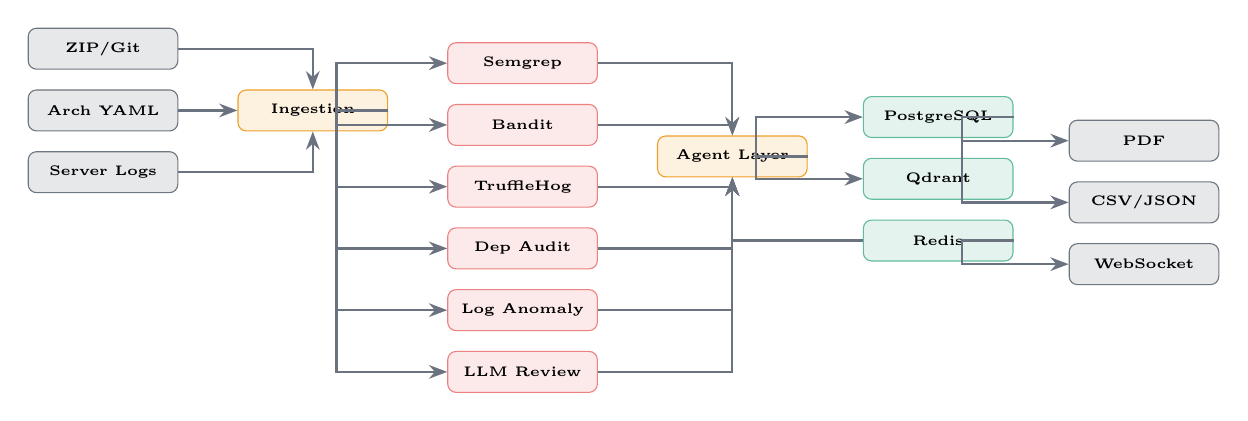
\begin{tikzpicture}[
  node distance=0.4cm and 0.75cm,
  box/.style={rectangle, rounded corners=3pt,
    minimum width=1.9cm, minimum height=0.52cm,
    draw, font=\tiny\bfseries, text centered},
  nbox/.style={box, fill=TLNavy!10, draw=TLNavy!60},
  rbox/.style={box, fill=TLRed!12, draw=TLRed!70},
  obox/.style={box, fill=TLOrange!15, draw=TLOrange},
  gbox/.style={box, fill=TLGreen!12, draw=TLGreen!70},
  arr/.style={-Stealth, thick, color=TLGray},
]
\node[nbox] (zip)  {ZIP/Git};
\node[nbox, below=0.25cm of zip]  (yaml) {Arch YAML};
\node[nbox, below=0.25cm of yaml] (logs) {Server Logs};
\node[obox, right=0.75cm of yaml] (ing)  {Ingestion};
\node[rbox, right=0.75cm of ing, yshift=0.6cm]  (sg)  {Semgrep};
\node[rbox, below=0.25cm of sg]   (ban)  {Bandit};
\node[rbox, below=0.25cm of ban]  (tfh)  {TruffleHog};
\node[rbox, below=0.25cm of tfh]  (dep)  {Dep Audit};
\node[rbox, below=0.25cm of dep]  (ano)  {Log Anomaly};
\node[rbox, below=0.25cm of ano]  (llm)  {LLM Review};
\node[obox, right=0.75cm of ban, yshift=-0.4cm] (agt) {Agent Layer};
\node[gbox, right=0.7cm of agt, yshift=0.5cm]   (pg)  {PostgreSQL};
\node[gbox, below=0.25cm of pg]   (qdr)  {Qdrant};
\node[gbox, below=0.25cm of qdr]  (red)  {Redis};
\node[nbox, right=0.7cm of pg, yshift=-0.3cm]   (pdf) {PDF};
\node[nbox, below=0.25cm of pdf]  (csv)  {CSV/JSON};
\node[nbox, below=0.25cm of csv]  (ws)   {WebSocket};
\draw[arr] (zip) -| (ing); \draw[arr] (yaml) -- (ing); \draw[arr] (logs) -| (ing);
\foreach \s in {sg,ban,tfh,dep,ano,llm} { \draw[arr] (ing) -- ++(0.3,0) |- (\s); }
\foreach \s in {sg,ban,tfh,dep,ano,llm} { \draw[arr] (\s) -| (agt); }
\draw[arr] (agt) -- ++(0.3,0) |- (pg);
\draw[arr] (agt) -- ++(0.3,0) |- (qdr);
\draw[arr] (red) -| (agt);
\draw[arr] (pg) -- ++(0.3,0) |- (pdf);
\draw[arr] (pg) -- ++(0.3,0) |- (csv);
\draw[arr] (red) -- ++(0.3,0) |- (ws);
\end{tikzpicture}}
\caption{ThreatLens layered pipeline architecture.}
\label{fig:arch}
\end{figure}

\subsection{Technology Stack}

\begin{table}[htbp]
\centering
\caption{ThreatLens Technology Stack}
\label{tab:stack}
\scriptsize
\begin{tabular}{@{}ll@{}}
\toprule
\textbf{Layer} & \textbf{Technology} \\
\midrule
API Server        & FastAPI 0.110 + Uvicorn (Python 3.11) \\
LLM Inference     & Groq API, Llama-3-70B \\
LLM Orchestration & LangChain 0.2 \\
Embeddings        & all-MiniLM-L6-v2 (384-dim) \\
Vector Store      & Qdrant (Docker, cosine) \\
Task Queue        & Celery 5.x + Redis 7 \\
Auth              & Supabase Auth + JWKS \\
Database          & PostgreSQL 15 + SQLAlchemy 2 + Alembic \\
Storage           & Supabase Storage (private buckets) \\
PDF Engine        & WeasyPrint 60 + Jinja2 3 + matplotlib 3.9 \\
Frontend          & TanStack Start + React 18 + TypeScript + Vite 5 \\
\bottomrule
\end{tabular}
\end{table}

\subsection{Repository Layout}
The backend resides in \texttt{threatlens/app/} across eleven
subdirectories: \texttt{auth/}, \texttt{models/}, \texttt{schemas/},
\texttt{api/}, \texttt{storage/}, \texttt{ingestion/}, \texttt{scanners/},
\texttt{rag/}, \texttt{agent/}, \texttt{report/}, and \texttt{tasks/}.

\section{RAG Compliance Knowledge Base}
\label{sec:rag}

\subsection{Corpus Composition}

\begin{table}[htbp]
\centering
\caption{RAG Corpus Composition}
\label{tab:corpus}
\scriptsize
\begin{tabular}{@{}llr@{}}
\toprule
\textbf{Framework} & \textbf{Chunk Unit} & \textbf{Chunks} \\
\midrule
GDPR             & Article               &  89  \\
SOC 2 Type II    & Common Criteria       &  67  \\
ISO 27001        & Annex A Control       & 114  \\
PCI DSS v4.0     & Requirement           & 156  \\
NIST CSF 2.0     & Subcategory           & 108  \\
\midrule
\textbf{Total}   &                       & \textbf{534} \\
\bottomrule
\end{tabular}
\end{table}

\subsection{Embedding and Vector Store}
ThreatLens uses \texttt{all-MiniLM-L6-v2}~\cite{reimers2019} (22M
parameters, 384-dim normalised dense vectors). The model is loaded once
at startup via the singleton pattern. Qdrant~\cite{qdrant} runs on
port~6333 with cosine distance; chunks are upserted in batches of 100.

\subsection{Retrieval}
At scan time the retriever embeds a finding's description text and
performs cosine similarity search optionally filtered to specific
frameworks. The top-12 most semantically similar control clauses are
prepended to the compliance mapper prompt.

\section{Scanner Layer}
\label{sec:scanners}

Six modules share a common interface: accept a filesystem path, return
normalised \texttt{FindingCreate} objects with severity, CWE identifier,
and file/line provenance. After parallel execution, findings are
deduplicated by the composite key (file\_path, line\_number, cwe\_id).

\textbf{Semgrep}~\cite{semgrep} runs eight rulesets (OWASP Top~10,
Python, JavaScript, secrets, JWT, SQL injection, XSS). Severity:
ERROR to Critical; WARNING to High; INFO to Medium.

\textbf{Bandit}~\cite{bandit} performs Python AST analysis detecting
subprocess.Popen(shell=True), hashlib.md5() without usedforsecurity=False,
and SQL string concatenation.

\textbf{TruffleHog v3}~\cite{trufflehog} uses entropy analysis and
verified pattern matching for 700+ credential types. Entropy thresholds:
hex above 3.0, base64 above 4.5. All findings: Critical severity, CWE-798.

\textbf{Dependency Audit}: pip-audit scans requirements.txt and
Pipfile.lock against OSV and NVD; npm audit scans package-lock.json and
yarn.lock.

\textbf{Log Anomaly}: brute-force detection (more than 50 failed auth
events per 5-min window), SQL injection in URLs via regex, unusual HTTP
methods. Additionally, IsolationForest(contamination=0.05) is applied to
a per-IP feature matrix of request rate, error rate, and endpoint
diversity.

\textbf{Groq Llama-3-70B Deep Review}: up to 30 source files sent to
Groq Llama-3-70B for contextual review. Files larger than 8 KB are
truncated. The model returns a validated JSON array; findings with
confidence below 0.70 are discarded.

\section{LangChain Agent Chains}
\label{sec:agent}

Four specialised LangChain~\cite{langchain} chains process each
deduplicated finding: RAG Retrieval (top-12 controls), Compliance Mapper
Chain, CVSS~3.1 Scorer Chain and Remediation Planner Chain in parallel,
then PostgreSQL Persistence, then Executive Summary Chain.

The \textbf{Compliance Mapper} retrieves top-12 control clauses from
Qdrant, constructs a grounded prompt, and invokes Groq Llama-3-70B.
Output is validated against the ComplianceMappingResult Pydantic schema.

\begin{lstlisting}[style=pycode, caption={Compliance mapper schema.}]
class FrameworkViolation(BaseModel):
    framework:             str
    control_id:            str
    violation_description: str
    evidence:              str

class ComplianceMappingResult(BaseModel):
    violations:           list[FrameworkViolation]
    cvss_score:           float   # 0.0-10.0
    cvss_vector:          str     # CVSS:3.1/AV:N/...
    remediation_steps:    list[str]
    remediation_priority: Literal[
        "immediate","short-term","long-term"]
\end{lstlisting}

The \textbf{CVSS~3.1 Auto-Scorer} evaluates eight CVSS metric dimensions
per the FIRST specification~\cite{CVSS31}, validated to [0.0, 10.0].
The \textbf{Remediation Planner} generates steps categorised as
Immediate (24 h), Short-term (1 week), or Long-term (1 month).
All Groq invocations use Tenacity exponential backoff
(stop\_after\_attempt(5), wait\_exponential(min=2, max=60)).
Prompt injection is mitigated by wrapping user code in explicit XML-style
delimiters.

\section{Report Generation and Export}
\label{sec:report}

PDF reports are generated through a three-stage pipeline:
(1) matplotlib renders a colour-coded compliance score bar chart
(green at least 80\%, orange 65--79\%, red below 65\%) as base64 PNG;
(2) Jinja2 assembles the report from modular templates;
(3) WeasyPrint~\cite{weasyprint} converts HTML to PDF.

PDFs are uploaded to private Supabase Storage buckets and served via
300-second signed URLs after workspace membership verification. CSV
(RFC~4180-compliant, with formula injection protection) and JSON exports
are also provided.

\section{Celery Task Pipeline}
\label{sec:task}

The scan lifecycle is managed by a single Celery task
\texttt{run\_full\_scan} with ten sequential phases.

\begin{table}[htbp]
\centering
\caption{Celery Scan Pipeline Phases}
\label{tab:celery}
\scriptsize
\begin{tabular}{@{}lll@{}}
\toprule
\textbf{Progress} & \textbf{Phase} & \textbf{Retries} \\
\midrule
0\%--5\%    & Initialisation     & 3 \\
5\%--15\%   & Ingestion          & 3 \\
15\%--30\%  & Semgrep            & 1 \\
30\%--40\%  & Bandit             & 1 \\
40\%--50\%  & TruffleHog         & 1 \\
50\%--70\%  & LLM Review         & 3 \\
70\%--75\%  & Deduplication      & 1 \\
75\%--95\%  & Compliance Mapping & 3 \\
95\%--100\% & Finalisation       & 1 \\
\bottomrule
\end{tabular}
\end{table}

Per-scanner failures are isolated: a Bandit failure on a non-Python
codebase logs the exception and continues with an empty findings list.
A Celery Beat schedule synchronises the NVD CVE corpus weekly (Sunday
02:00 UTC).

\section{Authentication and Multi-Tenancy}
\label{sec:auth}

Authentication is delegated to Supabase Auth~\cite{supabase}, managing
signup, PKCE OAuth flow, email verification, and token refresh. FastAPI
verifies JWTs against cached JWKS (5-minute TTL). All application
objects carry a workspace\_id foreign key. PostgreSQL RLS policies ensure
queries return only rows for workspaces where the session user holds
membership. Four roles are supported: Owner, Admin, Analyst, Viewer.

The slowapi middleware enforces per-user rate limits: 10 scan submissions
per hour, 5 report generations per hour, and 100 GET requests per minute.
The WebSocket channel requires an authentication message within five
seconds; the frontend falls back to 3-second TanStack Query polling on
connection failure.

\section{Empirical Evaluation}
\label{sec:eval}

\subsection{Test Environment}
Evaluation ran on NVIDIA RTX~4060 GPU (8 GB VRAM), 32 GB DDR5 RAM, 1 TB
NVMe SSD, with the backend in Docker (PostgreSQL~15, Redis~7, Qdrant).

\subsection{Scanner Detection Results}

\begin{table}[htbp]
\centering
\caption{Scanner Detection Results on Vulnerable Flask Fixture}
\label{tab:scanner}
\scriptsize
\begin{tabular}{@{}lcccc@{}}
\toprule
\textbf{Scanner} & \textbf{Expected} & \textbf{Detected} & \textbf{FP} & \textbf{Recall} \\
\midrule
Semgrep      & 12 & 11 & 2 & 91.7\% \\
Bandit       &  8 &  8 & 1 & 100\%  \\
TruffleHog   &  3 &  3 & 0 & 100\%  \\
Dep.\ Audit  &  3 &  3 & 0 & 100\%  \\
Log Anomaly  &  5 &  4 & 1 & 80.0\% \\
LLM Review   &  6 &  5 & 2 & 83.3\% \\
\midrule
\textbf{Total} & \textbf{37} & \textbf{34} & \textbf{6} & \textbf{91.9\%} \\
\bottomrule
\end{tabular}
\end{table}

\subsection{RAG Retrieval Precision}

\begin{table}[htbp]
\centering
\caption{RAG Retrieval Precision at $k{=}10$ by Framework}
\label{tab:rag}
\scriptsize
\begin{tabular}{@{}lccc@{}}
\toprule
\textbf{Framework} & \textbf{P@5} & \textbf{P@10} & \textbf{MR@1} \\
\midrule
GDPR         & 0.91 & 0.88 & 1.4 \\
SOC 2        & 0.89 & 0.86 & 1.6 \\
ISO 27001    & 0.93 & 0.89 & 1.2 \\
PCI DSS v4.0 & 0.88 & 0.84 & 1.7 \\
NIST CSF 2.0 & 0.90 & 0.87 & 1.5 \\
\midrule
\textbf{Mean} & \textbf{0.902} & \textbf{0.868} & \textbf{1.48} \\
\bottomrule
\end{tabular}
\end{table}

Mean P@10 of 0.868 demonstrates that all-MiniLM-L6-v2 is sufficiently
discriminative across five distinct regulatory vocabularies. MR@1 of 1.48
indicates a relevant control appears in the top two results in the
majority of queries.

\subsection{End-to-End Pipeline Performance}

\begin{table}[htbp]
\centering
\caption{Pipeline Phase Timing (47-file Codebase)}
\label{tab:perf}
\scriptsize
\begin{tabular}{@{}lrr@{}}
\toprule
\textbf{Phase} & \textbf{Time (s)} & \textbf{\%} \\
\midrule
Ingestion                     &  1.2 &  1.5 \\
Semgrep                       & 14.3 & 17.8 \\
Bandit                        &  3.1 &  3.9 \\
TruffleHog                    &  8.7 & 10.8 \\
Dependency Audit              &  6.2 &  7.7 \\
LLM Review (30 files, Groq)   & 28.4 & 35.4 \\
Deduplication                 &  0.3 &  0.4 \\
Compliance Mapping (34 items) & 17.6 & 21.9 \\
Report Generation             &  0.9 &  1.1 \\
\midrule
\textbf{Total}                & \textbf{80.7} & \textbf{100\%} \\
\bottomrule
\end{tabular}
\end{table}

LLM inference accounts for 57.3\% of total pipeline time (35.4\% deep
review + 21.9\% compliance mapping), confirming Groq API latency as the
dominant bottleneck.

\subsection{Test Suite Results}
The test suite achieves \textbf{89 passing, 4 skipped} across unit tests
for all eight implementation parts.

\section{Security Design}
\label{sec:security}

\begin{table}[htbp]
\centering
\caption{Security Mitigations by Threat Category}
\label{tab:security}
\scriptsize
\begin{tabular}{@{}lp{4.8cm}@{}}
\toprule
\textbf{Threat} & \textbf{Mitigation} \\
\midrule
Cross-tenant leakage
  & Supabase RLS on all tables; workspace\_id in every query; signed report URLs. \\
Prompt injection
  & Finding text wrapped in XML-style code delimiters. \\
ZIP bomb
  & Ratio check (at most 100x); max 1000 extracted files. \\
Path traversal
  & All extracted paths sanitised; patterns with ../ rejected. \\
Scanner code execution
  & No uploaded code is executed; subprocess envs stripped of credentials. \\
Subprocess timeout
  & 300 s hard timeout on all scanner subprocesses. \\
LLM hallucination
  & Pydantic strict-mode validation; malformed outputs discarded. \\
CSV formula injection
  & Cells starting with =, +, -, @ prefixed with a single quote. \\
Token leakage
  & WebSocket tokens in message body only, never in URL. \\
\bottomrule
\end{tabular}
\end{table}

Docker containers run as non-root users on python:3.11-slim. Celery uses
JSON serialisation (not pickle) to prevent deserialisation attacks.
Task results expire from Redis after 3600 seconds.

\section{Conclusion}
\label{sec:conclusion}

ThreatLens demonstrates that multi-tool static analysis, LLM-agentic
reasoning, and retrieval-augmented compliance mapping substantially
reduce the manual effort required for audit-ready security assessments.
The system achieves a 91.9\% aggregate detection rate, mean RAG
retrieval precision of 0.868 across five frameworks, and approximately
81 seconds end-to-end on a 47-file codebase.

Limitations include LLM latency (approximately 45 scans per hour per
Groq rate limit), a 16\% combined false-positive rate, compliance corpus
requiring periodic re-seeding, and no binary or container analysis.

Future work: CI/CD webhook integration; CodeQL taint-tracking; framework
expansion (HIPAA, SOX, FedRAMP, India DPDPA~2023); fine-tuned 7B
compliance LLM; automated remediation PR generation; GRC platform
integration (Drata, Vanta, Secureframe).

\section*{Acknowledgment}
The author thanks the project guide and faculty of the Department of
Computer Science and Engineering, G.~H.~Raisoni College of Engineering,
Nagpur. Gratitude is due to the open-source communities behind Semgrep,
Bandit, TruffleHog, LangChain, Qdrant, FastAPI, Supabase, and WeasyPrint.
The IEEE GHRCE Student Branch and Google Developer Groups On Campus GHRCE
provided valuable support.

\begin{thebibliography}{30}

\bibitem{GDPR2016}
European Parliament and Council of the EU,
``General Data Protection Regulation (GDPR): Regulation (EU) 2016/679,''
\textit{Official Journal of the European Union}, vol.~L~119, pp.~1--88, 2016.

\bibitem{PCIDSS4}
PCI Security Standards Council,
``PCI DSS Version 4.0,''
Technical Report, PCI SSC, Mar.~2022.

\bibitem{ISO27001}
International Organisation for Standardisation,
\textit{ISO/IEC~27001:2022 -- Information Security, Cybersecurity and
Privacy Protection},
ISO, Geneva, 2022.

\bibitem{NISTCSF2}
National Institute of Standards and Technology,
``The NIST Cybersecurity Framework 2.0,''
NIST Special Publication, Feb.~2024.

\bibitem{SOC2}
American Institute of Certified Public Accountants,
\textit{SOC~2 Type~II: Trust Services Criteria},
AICPA, 2022.

\bibitem{CVSS31}
P.~Mell and K.~Scarfone,
``A Complete Guide to the Common Vulnerability Scoring System Version 3.1,''
Technical Report, FIRST, Jun.~2019.

\bibitem{zhou2024llmvuln}
X.~Zhou et al.,
``LLM for Vulnerability Detection and Repair: Literature Review and Road Ahead,''
\textit{ACM Trans.\ Softw.\ Eng.\ Methodol.}, 2024, arXiv:2404.02525.

\bibitem{steenhoek2024finetune}
A.~Steenhoek et al.,
``Finetuning LLMs for Vulnerability Detection,''
\textit{IEEE Access}, 2024, arXiv:2401.17010.

\bibitem{fan2025dlvuln}
G.~Fan et al.,
``Deep Learning Aided Software Vulnerability Detection: A Survey,''
\textit{arXiv preprint arXiv:2503.04002}, 2025.

\bibitem{pearce2022asleep}
H.~Pearce et al.,
``Asleep at the Keyboard? Assessing the Security of GitHub Copilot's Code,''
in \textit{Proc.\ 43rd IEEE Symp.\ Security and Privacy}, pp.~754--768, 2022.

\bibitem{thakur2023}
A.~Thakur et al.,
``Enhancing Software Vulnerability Detection Using LLMs,''
\textit{arXiv preprint arXiv:2401.12169}, 2023.

\bibitem{lewis2020rag}
P.~Lewis et al.,
``Retrieval-Augmented Generation for Knowledge-Intensive NLP Tasks,''
in \textit{NeurIPS}, vol.~33, pp.~9459--9474, 2020.

\bibitem{pnnl2024cyrag}
Pacific Northwest National Laboratory,
``Retrieval Augmented Generation for Robust Cyber Defense (CyRAG),''
Technical Report, PNNL, 2024, arXiv:2402.14160.

\bibitem{veeraReddy2024}
S.~Veera Reddy and D.~Bhattacharyya,
``Hallucination Reduction in Compliance LLMs via RAG,''
\textit{Int.\ J.\ Intell.\ Syst.\ Appl.}, vol.~16, no.~3, pp.~45--59, 2024.

\bibitem{mauri2022stride}
L.~Mauri and E.~Damiani,
``Modeling Threats to AI-ML Systems Using STRIDE,''
\textit{Sensors (MDPI)}, vol.~22, no.~17, p.~6662, 2022.

\bibitem{setu2023secretbench}
S.~Setu et al.,
``SecretBench: A Dataset of Software Secrets,''
in \textit{Proc.\ 20th IEEE/ACM MSR}, pp.~403--414, 2023, arXiv:2303.06729.

\bibitem{ma2024seagull}
S.~Ma et al.,
``Flow-Aware Credential Leakage Detection (SEAGULL),''
\textit{IEEE Trans.\ Inf.\ Forensics Security}, 2024, arXiv:2403.00336.

\bibitem{meli2019}
M.~Meli et al.,
``How Bad Can It Git? Secret Leakage in GitHub Repositories,''
in \textit{Proc.\ NDSS}, 2019.

\bibitem{marandi2023devsecops}
M.~Marandi et al.,
``Automating Security Scanning in a DevSecOps CI/CD Pipeline,''
in \textit{IEEE WCONF}, pp.~1--6, 2023.

\bibitem{chua2024iforest}
W.~Chua et al.,
``Web Traffic Anomaly Detection Using Isolation Forest,''
\textit{Informatics (MDPI)}, vol.~11, no.~4, p.~83, 2024.

\bibitem{wang2024vulndeps}
J.~Wang et al.,
``Impact of Vulnerable Dependencies on Open-Source Software,''
in \textit{Proc.\ 35th IEEE ISSRE}, 2024, arXiv:2408.08472.

\bibitem{reimers2019}
N.~Reimers and I.~Gurevych,
``Sentence-BERT: Sentence Embeddings Using Siamese BERT-Networks,''
in \textit{Proc.\ EMNLP}, pp.~3982--3992, 2019.

\bibitem{semgrep}
Semgrep Open Source,
``Semgrep: Static Analysis at Ludicrous Speed,''
\url{https://semgrep.dev}, 2024.

\bibitem{bandit}
PyCQA Bandit Contributors,
``Bandit: A Security Linter for Python,''
\url{https://bandit.readthedocs.io}, 2024.

\bibitem{trufflehog}
Truffle Security Co.,
``TruffleHog v3: Secret Scanner with Verified Detectors,''
\url{https://github.com/trufflesecurity/trufflehog}, 2024.

\bibitem{qdrant}
Qdrant Solutions GmbH,
``Qdrant: Vector Similarity Search Engine,''
\url{https://qdrant.tech}, 2024.

\bibitem{langchain}
H.~Chase,
``LangChain: Building Applications with LLMs through Composability,''
\url{https://github.com/langchain-ai/langchain}, 2023.

\bibitem{fastapi}
S.~Ramirez,
``FastAPI: Modern Web Framework for Building APIs with Python 3.11+,''
\url{https://fastapi.tiangolo.com}, 2024.

\bibitem{supabase}
Supabase Inc.,
``Supabase: The Open-Source Firebase Alternative,''
\url{https://supabase.com}, 2024.

\bibitem{celery}
A.~Solem and Contributors,
``Celery: Distributed Task Queue,''
\url{https://docs.celeryq.dev}, 2024.

\bibitem{weasyprint}
Kozea SAS,
``WeasyPrint: The Awesome Document Factory,''
\url{https://weasyprint.org}, 2024.

\end{thebibliography}

\end{document}
